\section{From Write Admission to Retrieval Exposure}
\label{sec:admission}
The principal public-implementation experiment asks whether a bounded set of retrieved memories can safely stand in for the complete store when admitting repeated literal facts. We test the synchronous inferred-ingestion path of Mem0 at commit \texttt{26cdefb4}, whose package version is 2.2.1 \cite{mem0contributors2026oss}. The source retrieves at most ten write-time candidates, constructs its existing MD5-hash set from those candidates, suppresses hashes present in that set or already emitted within the current batch, and assigns fresh UUIDs to admitted records. This is an implementation observation, not a vendor promise of exactly-once ingestion.

\subsection{A conditional admission boundary}
Let $S$ contain $N$ distinct literal hashes already stored for the selected user, $V$ the retrieved candidates with $|V|\leq k$, and $X$ the distinct literal hashes emitted by extraction. Ignoring hash collisions, the tested admission rule suppresses $H(V)$ and within-batch repeats. The hashes of already stored facts that it may admit are therefore
\begin{equation}
 B=(X\cap S)\setminus H(V).
 \label{eq:admission}
\end{equation}
If extraction re-emits all of $S$, or at least every member of $S\setminus H(V)$, then
\begin{equation}
 |B|\geq\max(0,N-k).
 \label{eq:capacity}
\end{equation}
This is an elementary conditional counting argument. It is neither a new deduplication theorem nor a prediction that an arbitrary LLM will emit those facts. It identifies a precise obligation: a semantic candidate window does not establish global literal absence. Persisting a nondeterministic extraction result also does not make replay of its physical effects idempotent when admission assigns fresh addresses.

\subsection{Controlled native-pipeline experiment}
Before measured execution, we froze eight batch sizes ($1,5,10,11,13,20,21,40$), two explicit extraction controls, two embedding implementations, and three arms: $8\times2\times2\times3=96$ parameterized executions. Each execution invokes native \texttt{Memory.add} initially and twice more with the identical source, giving 288 calls. One extractor re-emits all literal facts; the other emits only facts absent from the visible candidate texts. Both are controlled callbacks, not measured LLM behavior, and deliberately do not use past messages for deduplication.

The embedding factor compares a nonsemantic hash control with actual local BGE-small-en-v1.5 inference (384 dimensions), through FastEmbed 0.9.1 and Qdrant-client 1.20.0 local mode \cite{baai2023bgesmall,qdrant2026fastembed,qdrant2026client}. The native arm retains $k=10$. An authored search wrapper widens that write-time request to 10,000; a separate authored sequential filter checks complete current-store exact text before returning extracted facts. These interventions are not stock Mem0 flags or atomic concurrent-admission fixes. Native storage and admission source remain unchanged. Telemetry is disabled; model files are prewarmed and measured controlled executions disallow external connections.

All 96 executions preserve the expected final literal fact set. For every native configuration with $N>10$, physical record counts are $N$, $2N-10$, and $3N-20$ across the three calls; the 40-fact case yields 40, 70, and 100 records (Figure~\ref{fig:admission}). All sizes at or below ten and both intervention arms admit no extra copies. Twenty of 32 native parameter cells have extra physical records. Repetition across controlled extractors and embedders establishes this finite mechanism under those configurations, not independent failure types or a population incidence estimate. A separate checker verifies every raw Qdrant/history store, admitted response, candidate set, and frozen source/specification identity.

\begin{figure}[t]
 \centering
 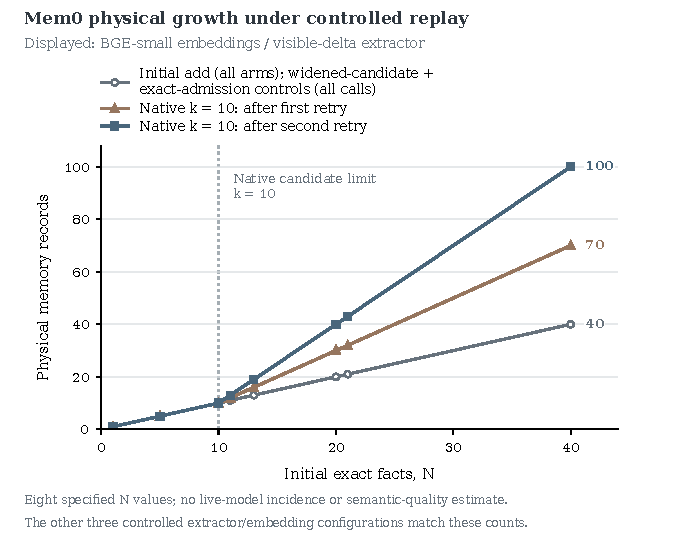
\includegraphics[width=0.92\linewidth]{figures/fig_mem0_bulk_replay.pdf}
 \caption{Controlled native Mem0 admission with real BGE embeddings and the visible-candidate extraction control. Initial calls and both intervention arms retain $N$ records; native exact-source redeliveries exceed $N$ above the ten-candidate boundary. The other three extractor/embedding combinations agree. These are parameterized controlled executions, not live-model failure-rate estimates.}
 \label{fig:admission}
\end{figure}

\subsection{Live extraction and actual process recovery}
A separate frozen protocol uses four authored source batches ($N=8,12,24,40$) and the native role-designated extraction prompts with requested Sol 6.1 through a personal Codex account \cite{openai2026codexexec}. Each baseline call commits native effects, returns from \texttt{Memory.add}, records an evaluator witness, and then actually exits its worker with \texttt{os.\_exit(87)} before logical acknowledgement. All four baselines extract and store exactly $N$ distinct facts and reach this exit. These are client/process cuts after effects, not network packet loss or storage mid-commit failure.

Fresh processes reopen copies of each baseline's native Qdrant/history state, preserving original record identities. Four batch sizes, two recent-message settings, three arms, and two extraction-recovery strategies give 48 retries. The fresh strategy makes 24 new model requests; the recorded-result strategy reuses the baseline response exactly and makes none. Together with four baseline requests, there are 28 actual requests. Every retry completes normally.

The recent-message settings retain native history or append twelve neutral messages so that the native last-ten-message window no longer contains the original source. Even the fresh-history prompt truncates each past message to 300 characters; the repeated new-source message remains complete. Native Summary and Recently Extracted Memories remain their default empty values in both settings; we do not disable a populated cache. These are explicit prompt/cache preconditions. They are not independently sampled conversational histories.

For each context setting, fresh-model native retries add $0,2,14,30$ records across the four sizes. In fresh history all 46 additions are exact baseline-text copies. In aged history 45 are exact copies and one is a new literal formulation, which we leave semantically ungraded. Thus the eight fresh-model native retries add 91 exact copies and one new string. Recorded-result native retries add 92 exact copies. Both interventions add zero records in all corresponding retries. Original identities and values survive in every arm. The one new formulation prevents treating Equation~\ref{eq:capacity} as a universal literal-count equality for fresh model output.

The evidence includes full native prompts, raw and used responses, candidate traces, request statuses and 52 raw baseline/retry stores. Configuration injection changes the extraction provider, not native admission source. The requested alias, CLI version and visible usage are retained; the exact backend model snapshot, harness system prompt, temperature and seed are not exposed or controlled. This is one model/harness and four source batches, not a model comparison, semantic error rate or natural-workload estimate.

\subsection{Target presence can coexist with redundant context}
After observing the live writes, we froze a post hoc exposure protocol before issuing its measured queries. It uses every distinct baseline fact as a literal query (84 across the four sizes), four store states (baseline and each fresh-history/fresh-model retry arm), and retrieval budgets $K\in\{5,10,20\}$: $84\times4\times3=1008$ native \texttt{Memory.search} calls. All states use the same reader, BGE/BM25 configuration, zero score threshold, and \texttt{show\_expired=False}. Optional spaCy is absent and the native fallback is used. The write-time candidate bound $k=10$ and reader budget $K$ are different parameters.

The fresh-history states hold literal content and original identities fixed; every added point is an exact baseline-text copy, with its BGE vector matching within $10^{-6}$. This deliberate selection excludes the aged retry's ungraded formulation. It is a mechanism probe, not held-out generalization. Define per-query returned slots $r_q$, distinct literal strings $u_q$, duplicate slots $d_q=r_q-u_q$, and exact target presence $t_q$. All 1008 queries have $t_q=1$. Nevertheless, at $N=40,K=10$, native retries return 400 slots with only 247 summed per-query distinct strings, versus 400 distinct strings in baseline and each intervention. The 153 duplicate slots reduce mean distinct strings per query from 10 to 6.175 (minimum 5); Figure~\ref{fig:exposure} shows all four sizes.

\begin{figure}[t]
 \centering
 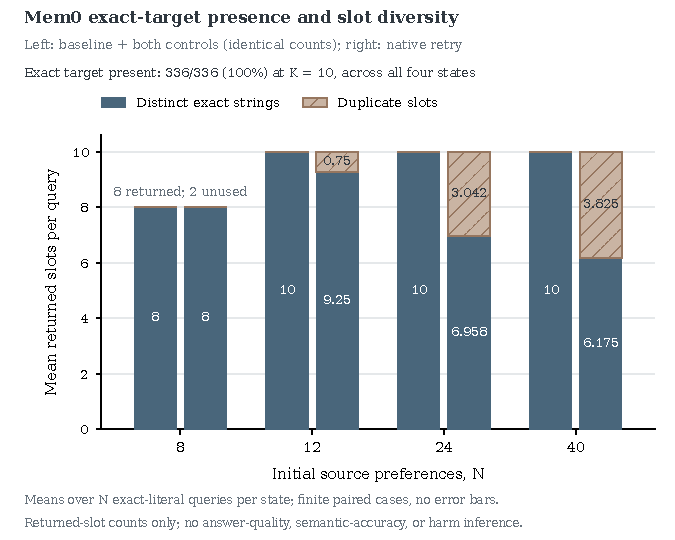
\includegraphics[width=0.92\linewidth]{figures/fig_mem0_retrieval_slots.pdf}
 \caption{Retrieval exposure at budget ten across all four authored batch sizes. Bars separate distinct exact strings from duplicate slots, averaged over every baseline-fact query. Both intervention states match baseline. Every exact target is present. Distinct literal strings are not semantic diversity or answer quality; unused capacity for batches smaller than the budget is not duplication.}
 \label{fig:exposure}
\end{figure}

Across all budgets, 213 query cells contain duplicate slots, but only 201 have fewer distinct strings than matched baseline. For $N=12,K=20$, duplicate records occupy previously spare capacity without reducing the twelve distinct strings. Thus duplication and displaced evidence must be checked separately. No answer-generation task, downstream harm, semantic relevance annotation, latency or token-cost measurement is performed.

A separately implemented checker reconstructs coverage, raw identities/vectors/history, query results and paired metrics. The original runner deletes its temporary reader copies, so a frozen retention wrapper repeats the same computation and retains all sixteen after-close stores. All 1008 ordered result-identity lists and metrics match; retained point blobs/history are unchanged. This is computational reproduction by the same study, not 1008 additional independent samples. The empirical contribution is the conjunction of a bounded admission witness, native live recovery evidence, and measured context redundancy despite perfect exact-target presence.
